\documentclass[tikz, border=1cm]{standalone}
\usetikzlibrary{intersections, ext.paths.arcto}
\begin{document}
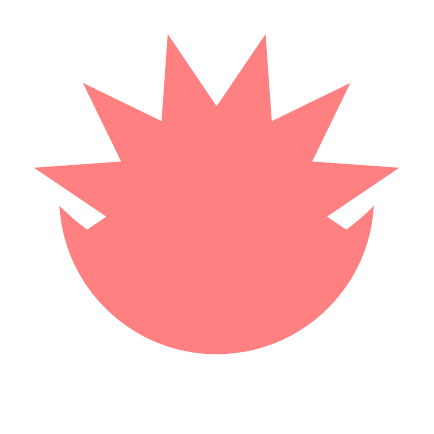
\begin{tikzpicture}

\pgfmathsetmacro{\teeth}{12}
\pgfmathsetmacro{\innerR}{1.4}
\pgfmathsetmacro{\outerR}{2.4}
\draw[draw=none,save path=\star] (0:\innerR) \foreach \i in {1,...,\teeth} {-- ({(\i-0.5)*360/\teeth}:\outerR) -- (\i*360/\teeth:\innerR)} -- cycle;

\pgfmathsetmacro{\radA}{2.0}
\pgfmathsetmacro{\radB}{2.8}
\coordinate (A) at (0,0.25);
\coordinate (B) at (0,2.1);
\path[name path=CA, overlay] (A) circle (\radA);
\path[name path=CB, overlay] (B) circle (\radB);
\path[name intersections={of=CA and CB, by={I1,I2}}];
\draw[draw=none,save path=\moon] (I1) arc to[radius=\radA] (I2) arc to[radius=\radB,clockwise](I1) -- cycle;

\begin{scope}
\clip (\outerR,-\outerR) rectangle (-\outerR,\outerR) (-\outerR,-\outerR) -- (-\outerR,0) -- (I1) arc to[radius=0.5*(\radA+\radB)] (I2) -- (\outerR,0) -- (\outerR,-\outerR) -- cycle; %replace \clip with \fill[red] to see area
\fill[red!50, use path=\star];
\end{scope}
\fill[red!50, use path=\moon];

\end{tikzpicture}
\end{document}